%!TEX root = ../../super_main.tex

\section{Snapshot}
\label{sec:snapshot}

% Motivation 
We will also need a model for the gathered data to complement the specifications of how the individual snapshots should be composed. This model should be able handle different types of data from different sensors. Some measurements will be simple floating point numbers, to approximate real numbers, and others will consist of more complex types aggregating different values possibly of different types.  

\section{FloatTriple}
We should minimize the required storage footprint of the collected data from the data collecting application in order to minimize power consumption and thereby affecting other use of applied mobile devices as little as possible as described in \secref{sec:start_configuration}. We have for this reason designed a concept called FloatTriple. A FloatTriple is an object which is used to compress three floats into the size of long, meaning we convert 12 bytes (three times 4 bytes) to be stored in 8 bytes. We do this by ABANDONNING some of the precision of a float.
\\\\
When compressing three floats into a FloatTriple we assumes that the SAGERFØRKOMMA will never exceed 8, because most of our sensors produce values ranging from -360 to 360. We strip the decimal separator from the floats an treat them as a 20 bit integer value, where the first bit determines whether the value is positive or negative. We now use 60 bit for storing the compressed value of the floats. Furthermore, we add 3 bits for representing where the decimal should be placed in the floats. How we compress the floats to a long and what the bit string of our FloatTriple represents can be seen in \figref{fig:float_triple_convert} and \figref{fig:float_triple_bit} respectively.
\begin{figure}[!htbp]
    \begin{alignat*}{6}
       &8.138   &&                   &&   && 8138  &&                   && \text{\mono{00000001111111001010}} \\
      -&12.821  && ~~ \rightarrow ~~ && - && 12821 && ~~ \rightarrow ~~ && \text{\mono{10000011001000010101}} \\
       &42.4878 &&                   &&   && 42487 &&                   && \text{\mono{00001010010111110111}} 
    \end{alignat*}
    \caption{Compression of floats.}
    \label{fig:float_triple_convert}
\end{figure}

\begin{figure}[!htbp]
    \centering
    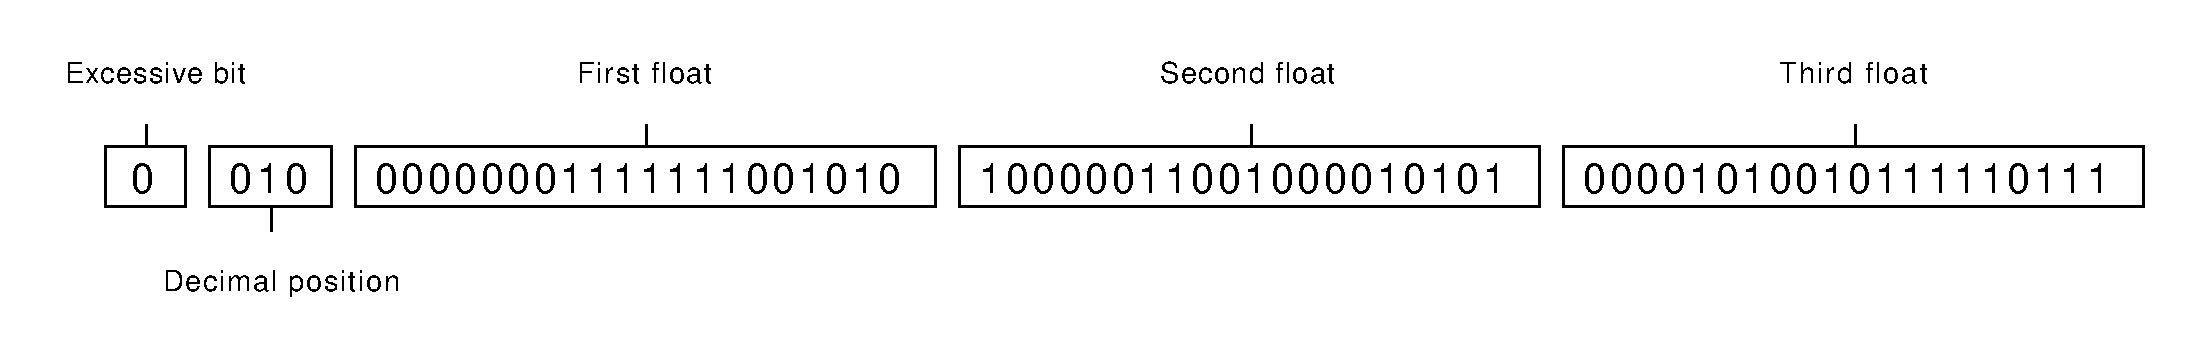
\includegraphics[width=\textwidth]{graphic/data_modeling/float_triple_bit.pdf}
    \caption{The bit representation of a FloatTriple.}
    \label{fig:float_triple_bit}
\end{figure}
We wanted to compress the floating point values of the sensors so that the size of the data we need to send over network and store on the device would decrease. However, this compression does not come for free. We actively trade off size of data stored and send with CPU cycles for compressing and decompressing the values. 
\todo[inline]{Insert test af performance}